% MyHatTileStuff/composing.c — Detailed Technical Explanation
% Compile with: pdflatex -shell-escape composing.tex
%
\documentclass[10pt,a4paper]{article}

%% ---------- Packages ----------
\usepackage[T1]{fontenc}
\usepackage[utf8]{inputenc}
\usepackage{geometry}
\geometry{margin=2cm, top=2.2cm, bottom=2.5cm}

\usepackage{microtype}
\usepackage{parskip}
\usepackage{xcolor}
\usepackage{booktabs}
\usepackage{amsmath,amssymb}
\usepackage{graphicx}
\usepackage{hyperref}
\usepackage{enumitem}
\setlist{noitemsep, topsep=2pt}
\usepackage{needspace}

%% minted — syntax highlighting (requires -shell-escape and pygments)
\usepackage{minted}
\setminted{
  fontsize=\footnotesize,
  baselinestretch=1.1,
  breaklines=true,
  linenos=false,
  frame=none,
  bgcolor=codebg
}
\definecolor{codebg}{HTML}{F5F5F5}

%% tcolorbox — outlined panels
\usepackage[most]{tcolorbox}
\tcbuselibrary{minted,skins,breakable}

%% Colours
\definecolor{titlecolor}{HTML}{1A4D8F}
\definecolor{headercolor}{HTML}{2E6DB4}
\definecolor{rulecolor}{HTML}{AECBEF}
\definecolor{seedorange}{HTML}{F39C12}
\definecolor{seedred}{HTML}{E74C3C}
\definecolor{seedpurple}{HTML}{8E44AD}
\definecolor{centerred}{HTML}{C0392B}

%% Section colours
\usepackage{titlesec}
\titleformat{\section}{\large\bfseries\color{titlecolor}}{}{0em}{}[\nobreak\vspace{-2pt}\color{rulecolor}\hrule\nobreak\vspace{4pt}]
\titleformat{\subsection}{\normalsize\bfseries\color{headercolor}}{}{0em}{}

%% Keep headings attached to the content that follows them
\newcommand{\subsectionbreak}{\nobreak}
\let\polysection\section
\renewcommand\section{\needspace{0.16\textheight}\polysection}
\let\polysubsection\subsection
\renewcommand\subsection{\needspace{0.12\textheight}\polysubsection}

%% Convenient macros
\newcommand{\code}[1]{\texttt{\small #1}}
\newcommand{\file}[1]{\texttt{\footnotesize #1}}
\newcommand{\vcoord}[3]{$(#1,\,#2,\,#3)$}

%% Side-by-side panes are built from two minipages inline in the body.
%% (minted cannot be passed as a macro argument, so no wrapper command.)
\newcommand{\panegap}{\hfill}

%% ---------- Document ----------
\begin{document}

\begin{center}
  {\Huge\bfseries\color{titlecolor} composing.c}\\[4pt]
  {\large\color{headercolor} Three Hat Tiles Sharing the Central Vertex $v[12]$}\\[6pt]
  {\small \file{MyHatTileStuff/composing.c} — Technical Reference}\\[2pt]
  {\small\color{gray} \today}
\end{center}

\vspace{6pt}
\noindent\rule{\linewidth}{1pt}
\vspace{4pt}

% -----------------------------------------------------------------------
\section{Purpose}

\code{composing} builds a single static figure: three copies of the hat tile
arranged as a \emph{pinwheel} around one shared vertex.  The base hat is
placed at orientation $0^\circ$; two further copies are rotated by $120^\circ$
and $240^\circ$; and all three are positioned so that vertex \code{v[12]} of
every copy lands on exactly the same lattice point.  The result is rendered to
\file{img/composing.svg}.

\medskip
\noindent Unlike its larger sibling \code{grow\_symmetric2} (which grows
clusters ring-by-ring under the RL0 rulebook), \code{composing} does
\emph{no} rule-based growth.  It is a focused geometric construction:
rotate, attach, verify the shared vertex, draw.  This makes it an ideal
program for studying the attachment primitives and the C calling
conventions they rely on.

% -----------------------------------------------------------------------
\section{Data Types}

Four small structs from \file{core/cycle.h} drive the whole program.  Their
sizes matter for the discussion of pointer arguments in
Section~\ref{sec:amp}.

\begin{minted}{c}
typedef struct { int v; int x; int y; } Coord;          /* a lattice point (12 bytes) */
typedef struct { int n; Coord v[MAX_VERTS]; } Cycle;    /* a polygon boundary (large) */
typedef struct { int cycle_count; Cycle cycles[MAX_CYCLES]; } Poly; /* >=1 cycles (very large) */
typedef struct { Coord a; Coord b; } Edge;              /* an oriented boundary edge */
\end{minted}

\noindent A \code{Coord} is a tagged lattice point: \code{v} is the valence
tag ($6$, $4$ or $3$) and $(x,y)$ are integer coordinates.  A \code{Cycle}
holds up to \code{MAX\_VERTS}~$=384$ vertices, so it is several kilobytes
wide; a \code{Poly} holds up to \code{MAX\_CYCLES}~$=32$ such cycles and is
larger still.  These size facts are exactly why the library passes
\code{Cycle} and \code{Poly} \emph{by pointer} while it passes \code{Coord}
\emph{by value}.

% -----------------------------------------------------------------------
\section{Program Walkthrough}

\subsection{Setup: load and rotate}

\par\medskip\noindent
\begin{minipage}[t]{0.46\linewidth}
\setlength{\parskip}{4pt}
The tile is read from \file{tiles/hat.tile} into a \code{Tile} struct.
(The file header comment mentions \file{preferences/focus.tile}; the code
actually loads \file{tiles/hat.tile}.)

Three orientations are produced.  \code{rot[0]} is the base hat as loaded.
\code{cycle\_transform\_lattice} applies the exact origin-centred
$60^\circ$-step lattice rotation; $t=2$ gives $120^\circ$ and $t=4$ gives
$240^\circ$.

The shared centre is read off the \emph{base} hat:
\code{center = tile.base.v[12]}, namely \vcoord{3}{1}{-1}.
\end{minipage}\panegap
\begin{minipage}[t]{0.50\linewidth}
\begin{minted}{c}
Tile tile;
tile_load("tiles/hat.tile", &tile);

Cycle rot[NUM_HATS];          /* NUM_HATS = 3 */
rot[0] = tile.base;
cycle_transform_lattice(&tile.base,
        &rot[1], tile.lattice, 2);   /* 120 deg */
cycle_transform_lattice(&tile.base,
        &rot[2], tile.lattice, 4);   /* 240 deg */

Coord center = tile.base.v[CENTER_VERTEX];
/* CENTER_VERTEX = 12 -> (3,1,-1) */
\end{minted}
\end{minipage}
\par\medskip

\subsection{Seed: the first hat}

The growing figure is tracked in two parallel arrays.  \code{hats[k]} stores
the placed hat \emph{cycle} (for drawing); \code{poly[k]} stores the merged
\emph{polygon} after $k+1$ hats have been glued together (for the next
attachment).  Hat~0 seeds both:

\begin{minted}{c}
Poly  poly[NUM_HATS];
Cycle hats[NUM_HATS];
hats[0]             = rot[0];
poly[0].cycle_count = 1;
poly[0].cycles[0]   = rot[0];
\end{minted}

% -----------------------------------------------------------------------
\section{The Attachment Loop}
\label{sec:loop}

This is the heart of the program: it glues hat~1 and then hat~2 onto the
figure, insisting each time that the new copy's \code{v[12]} fall on the
shared centre.

\par\medskip\noindent
\begin{minipage}[t]{0.46\linewidth}
\setlength{\parskip}{4pt}
\textbf{Outer loop — \code{k = 1, 2}.}  At the start of iteration \code{k}
the figure \code{poly[k-1]} already contains \code{k} hats.  We attach
\code{rot[k]} to it.  \code{build\_boundary\_edges} fills \code{edges[]}
with the outline of \code{poly[k-1]} and returns the edge count \code{ec}.

\textbf{Search loops — \code{be}, \code{te}.}  We try gluing the new tile
along every \emph{base} boundary edge \code{be} ($0\ldots ec$) against
every \emph{tile} edge \code{te} ($0\ldots\code{rot[k].n}$).  Both loops
carry the guard \code{\&\& !ok}, so the search stops the instant a valid
placement is accepted.

\textbf{Acceptance — three tests.}  A candidate placement must pass all of:
\begin{enumerate}
  \item \code{try\_attach\_tile\_poly\_ex} returns non-zero — the tile fits
    along $(be,te)$ without overlap, yielding the merged polygon \code{out}
    and the placed cycle \code{aligned}.
  \item \code{out.cycle\_count == 1} — the merge produced no holes.
  \item \code{coord\_eq(aligned.v[12], center)} — the new copy's vertex 12
    sits on the shared centre.
\end{enumerate}
Test~3 is what makes this a pinwheel rather than an arbitrary
edge-to-edge join.  On success we record \code{hats[k]} and \code{poly[k]}
and set \code{ok = 1}; if no $(be,te)$ works the program reports an error
and exits.
\end{minipage}\panegap
\begin{minipage}[t]{0.50\linewidth}
\begin{minted}{c}
Edge edges[512];
for (int k = 1; k < NUM_HATS; k++) {
    int ok = 0;
    int ec = build_boundary_edges(
                 &poly[k-1], edges);
    for (int be = 0; be < ec && !ok; be++) {
      for (int te = 0;
           te < rot[k].n && !ok; te++) {
        Poly  out;
        Cycle aligned;
        if (!try_attach_tile_poly_ex(
                &poly[k-1], &rot[k],
                tile.lattice, be, te,
                &out, &aligned))
            continue;
        if (out.cycle_count > 1) continue;
        if (!coord_eq(aligned.v[CENTER_VERTEX],
                      center))   continue;
        hats[k] = aligned;   /* keep cycle  */
        poly[k] = out;       /* keep merge  */
        ok = 1;
      }
    }
    if (!ok) { /* cannot attach */ return 1; }
}
\end{minted}
\end{minipage}
\par\medskip

\noindent The \code{edges[512]} buffer is allocated once, outside the loop,
and reused on every iteration: \code{build\_boundary\_edges} overwrites it
each time and returns the current length, so stale entries past \code{ec}
are simply never read.

% -----------------------------------------------------------------------
\section{The Ampersand (\&): Pass-by-Pointer in C}
\label{sec:amp}

The two calls inside the loop raise a natural question:

\begin{quote}
Why is there \emph{no} \code{\&} on \code{edges} in
\code{build\_boundary\_edges(\&poly[k-1], edges)}, but there \emph{is} a
\code{\&} on \code{aligned} in
\code{try\_attach\_tile\_poly\_ex(\ldots, \&aligned)}?
\end{quote}

\subsection{What \texttt{\&} does}

C passes every argument \emph{by value} — the function receives a private
copy.  To let a function write back into a caller's variable (an
\emph{output parameter}), or to avoid copying a large struct, you pass a
\emph{pointer} to it.  The unary \code{\&} (``address-of'') operator turns
an object into a pointer to that object: if \code{aligned} has type
\code{Cycle}, then \code{\&aligned} has type \code{Cycle *}.  The relevant
signatures are:

\begin{minted}{c}
int build_boundary_edges (const Poly *p, Edge *edges);
int try_attach_tile_poly_ex(const Poly *base, const Cycle *tile_variant,
                            int lattice, int base_edge_index, int tile_edge_index,
                            Poly *out, Cycle *aligned_out);
int coord_eq(Coord a, Coord b);   /* note: by value, no pointer */
\end{minted}

\subsection{The key rule: arrays decay, scalars/structs do not}

\par\medskip\noindent
\begin{minipage}[t]{0.46\linewidth}
\setlength{\parskip}{4pt}
\textbf{\code{aligned} needs \code{\&}.}  It is declared
\code{Cycle aligned;} — a \emph{single struct object}.  Its name has type
\code{Cycle}, but the parameter \code{aligned\_out} wants a \code{Cycle *}.
A lone struct does not turn itself into a pointer, so you must apply
\code{\&} explicitly: \code{\&aligned} is the \code{Cycle *} the function
writes its result through.  The same holds for \code{\&out} (a \code{Poly})
and for \code{\&poly[k-1]} (a \code{Poly} array \emph{element} — one
struct, hence \code{\&}).

\textbf{\code{edges} needs no \code{\&}.}  It is declared
\code{Edge edges[512];} — an \emph{array}.  In C an array name used in an
expression \emph{decays} to a pointer to its first element: \code{edges}
already has type \code{Edge *}, exactly what the parameter wants.  Adding
\code{\&} would give \code{\&edges} of type \code{Edge (*)[512]}
(pointer-to-array-of-512) — a different, wrong type that the compiler
would reject.
\end{minipage}\panegap
\begin{minipage}[t]{0.50\linewidth}
\begin{minted}{c}
/* single struct objects -> take address */
Poly  out;        /* &out     : Poly  *  */
Cycle aligned;    /* &aligned : Cycle *  */
poly[k-1];        /* &poly[k-1] : Poly * */

/* array object -> already a pointer */
Edge edges[512];  /* edges    : Edge  *  */
                  /* &edges : Edge (*)[512]  WRONG */

build_boundary_edges(&poly[k-1], edges);
/*                   ^struct     ^array  */

try_attach_tile_poly_ex(&poly[k-1], &rot[k],
        tile.lattice, be, te, &out, &aligned);
/*      ^struct   ^elem        ^out ^struct  */
\end{minted}
\end{minipage}
\par\medskip

\subsection{Both are still ``output parameters''}

The distinction is purely about \emph{type}, not intent.  Both \code{edges}
and \code{aligned} are written \emph{by} the callee and read \emph{by} the
caller afterwards.  \code{build\_boundary\_edges} fills \code{edges[0..ec-1]}
and returns \code{ec}; \code{try\_attach\_tile\_poly\_ex} fills \code{*out}
and \code{*aligned\_out} and returns a success flag.  The only reason one
gets a \code{\&} and the other does not is that an array hands you a pointer
for free, while a single struct does not.

\subsection{Contrast: passing by value}

The acceptance test uses \code{coord\_eq(aligned.v[12], center)} with
\emph{no} ampersands.  \code{coord\_eq} takes two \code{Coord} arguments
\emph{by value}: a \code{Coord} is only 12 bytes, so copying it is cheap and
the function has no need to modify the caller's data — it just reports
equality.  The general pattern across the codebase is therefore:

\begin{center}
\begin{tabular}{@{}lll@{}}
\toprule
\textbf{Object} & \textbf{How it is passed} & \textbf{At the call site} \\
\midrule
\code{Coord} (small, read-only) & by value          & bare: \code{center} \\
\code{Cycle} / \code{Poly} (large, or written) & by pointer & \code{\&aligned}, \code{\&out} \\
\code{Edge edges[512]} (array)  & decays to pointer & bare: \code{edges} \\
\bottomrule
\end{tabular}
\end{center}

\subsection{Argument-by-argument summary}

\begin{center}
\begin{tabular}{@{}llll@{}}
\toprule
\textbf{Call site arg} & \textbf{Declared as} & \textbf{Parameter type} & \textbf{Why} \\
\midrule
\code{\&poly[k-1]} & \code{Poly poly[3]} (element) & \code{const Poly *} & struct $\Rightarrow$ take address \\
\code{edges}       & \code{Edge edges[512]}        & \code{Edge *}       & array decays, no \code{\&} \\
\code{\&rot[k]}    & \code{Cycle rot[3]} (element) & \code{const Cycle *}& struct $\Rightarrow$ take address \\
\code{\&out}       & \code{Poly out}               & \code{Poly *}       & struct out-param $\Rightarrow$ \code{\&} \\
\code{\&aligned}   & \code{Cycle aligned}          & \code{Cycle *}      & struct out-param $\Rightarrow$ \code{\&} \\
\code{center}      & \code{Coord center}           & \code{Coord} (value)& small struct, by value \\
\bottomrule
\end{tabular}
\end{center}

% -----------------------------------------------------------------------
\section{SVG Rendering}

After the three hats are placed, \code{main} computes a bounding box over all
\code{hats[k].v[i]}, picks a pixel scale \code{SC = 50} and margin
\code{M = 24}, and writes the SVG.  Tetrille coordinates $(v,x,y)$ are mapped
to screen space by \code{svgx}/\code{svgy} (with $\sqrt 3$ pre-computed in
\code{g\_r3}):

\[
  (x_s,\,y_s) =
  \begin{cases}
    \bigl(\tfrac{\sqrt3}{2}(x+y),\ \tfrac12(y-x)\bigr) & v = 6 \\[3pt]
    \bigl(\tfrac{\sqrt3}{4}(x+y),\ \tfrac14(y-x)\bigr) & v = 4 \\[3pt]
    \bigl(\tfrac{x+\frac12 y}{\sqrt3},\ \tfrac12 y\bigr) & v = 3
  \end{cases}
\]

\noindent SVG's $y$-axis points down, so the draw routine emits
$y_{\text{svg}} = o_y - \texttt{SC}\cdot y_s$.  The three hats are filled in
amber, red and purple; a small dark-red disc and a \code{v[12]} text label
mark the shared centre.

\begin{center}
\begin{tabular}{@{}lll@{}}
\toprule
\textbf{Element} & \textbf{Colour} & \textbf{Hex} \\
\midrule
Hat 0 (base, $0^\circ$)   & {\color{seedorange}\rule{1em}{0.8em}} Amber  & \texttt{\#f39c12} \\
Hat 1 ($120^\circ$)       & {\color{seedred}\rule{1em}{0.8em}} Red    & \texttt{\#e74c3c} \\
Hat 2 ($240^\circ$)       & {\color{seedpurple}\rule{1em}{0.8em}} Purple & \texttt{\#8e44ad} \\
Shared vertex marker      & {\color{centerred}\rule{1em}{0.8em}} Dark red & \texttt{\#c0392b} \\
\bottomrule
\end{tabular}
\end{center}

\subsection{The Generated Figure}

\noindent The output \file{img/composing.svg} (converted here to PDF for
inclusion) shows the three hats meeting at the shared vertex
\code{v[12]}, namely \vcoord{3}{1}{-1}, marked by the dark-red disc:

\begin{center}
  \fbox{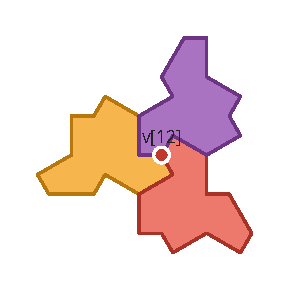
\includegraphics[width=0.42\linewidth]{composing_figure.pdf}}
\end{center}

\noindent\textit{To regenerate:} run \code{./bin/composing} from the project
root (writes \file{img/composing.svg}), then convert with
\code{inkscape img/composing.svg --export-type=pdf
--export-filename=manual/details/composing\_figure.pdf}.

% -----------------------------------------------------------------------
\section{Architecture Summary}

\begin{center}
\begin{tcolorbox}[
  colframe=rulecolor, colback=white, boxrule=0.6pt, arc=3pt,
  width=0.98\linewidth
]
\begin{minted}{text}
main()
  +-- tile_load("tiles/hat.tile", &tile)
  |
  +-- rot[0]=base, rot[1]=t2(base) [120deg], rot[2]=t4(base) [240deg]
  +-- center = tile.base.v[12] = (3,1,-1)
  +-- poly[0]/hats[0] = rot[0]
  |
  +-- for k=1,2:                               (the attachment loop)
  |     build_boundary_edges(&poly[k-1], edges) -> ec
  |     for be in 0..ec, te in 0..rot[k].n:
  |       try_attach_tile_poly_ex(&poly[k-1],&rot[k],..,&out,&aligned)
  |       require out.cycle_count==1
  |       require coord_eq(aligned.v[12], center)
  |       -> hats[k]=aligned, poly[k]=out
  |
  +-- bounding box over hats[*].v[*]  ->  SC=50, M=24
  +-- draw_hat x3 (amber / red / purple)
  +-- centre disc + "v[12]" label
  +-- write img/composing.svg
\end{minted}
\end{tcolorbox}
\end{center}

% -----------------------------------------------------------------------
\section{Usage}

\begin{minted}{bash}
# Build (Makefile or CMake target name: composing)
make composing

# Run from the project root (relative paths to tiles/ and img/)
./bin/composing
# -> writes img/composing.svg, prints "Wrote img/composing.svg"
\end{minted}

\medskip
\noindent\textbf{Working directory matters.}  \code{main} uses the relative
paths \file{tiles/hat.tile} and \file{img/composing.svg}, so the program
must be launched from the project root.  In CLion, set the run
configuration's \emph{Working directory} to the project root accordingly.

\vspace{4pt}
\noindent\rule{\linewidth}{0.6pt}
\vspace{2pt}

{\small\color{gray}
\file{MyHatTileStuff/composing.c} — part of PolyformTown.
Compile this document with \texttt{pdflatex -shell-escape composing.tex}
(requires \texttt{pygments} for \texttt{minted}).
}

\end{document}
